\documentclass[crop,tikz]{standalone}
\usepackage{circuitikz}
\begin{document}
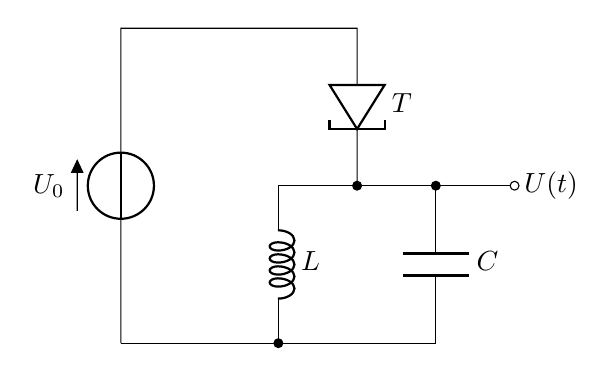
\begin{tikzpicture}
    \draw (2,2) to[L=$L$, n=l1, -*] (2,0);
    \draw (4,2) to[C=$C$, n=c1] (4,0);
    \draw (0,0) to[V=$U_0$, n=u0] (0,4) --
    	(3,4) to[tDo, l=$T$, -*, n=t1] (3,2);
    \draw (2,2)--(4,2);
    \draw (0,0)--(4,0);
    \draw (4,2) to[short,*-o] (5,2) node[right] {$U(t)$};
\end{tikzpicture}
\end{document}
